\chapter{Performance Comparison and Evaluation}
In this chapter, we describe our experiments regarding 2 research questions we proposed in chapter 1. The experiments based on the DevOps toolchains we implemented in Chapter 4. 
\par
In the Section 5,1, we will examine how does the serverless compute engine for containers (Amazon ECS on AWS Fargate) could influence the performance of an non+integrated toolchains. Thus in this experiment, we also implement the solution with a different type of cloud environment (with/without serverless) as a comparison group. 
In section 5.2, we focuses on answering research question 2, in which we will compare the performance of continuous delivery pipeline composed of fully-managed serverless DevOps tools in AWS with our Jenkins-based pipeline that runs on the virtual machine.
\section{Experiment on Serverless Container Services}
The Docker agent has already been supported by many CI/CD tools, for example container job\footnote{https://docs.microsoft.com/en-us/azure/devops/pipelines/process/container-phases} in Azure DevOps\footnote{https://azure.microsoft.com/en-us/services/devops/}, Docker agent in TeamCity \footnote{https://www.jetbrains.com/help/teamcity/build-agent.html}, Docker agent\footnote{https://www.jenkins.io/doc/book/pipeline/docker/} in Jenkins and docker runner\footnote{https://docs.drone.io/runner/docker/overview/} in Drone\footnote{https://drone.io/}
\par
The serverless container services in AWS (AWS Fargate) provides possibility to further ease the infrastructure management task for the Docker build agents. 
This experiment is a controlled experiment which examines whether serverless container service could improve the continuous delivery pipeline from various perspectives.
\subsection{Test Task and System Description}
In this experiment, we run the continuous delivery process of a Spring Boot web application with our DevOps toolchain. From the experiments, we could verify our assumption in CH3, and better-answering research question 1.
\par
As we described in Chapter 4, the continuous delivery pipeline includes the following steps:
\begin{enumerate}
    \item \textit{Checkout}: Pull the most recent change from Github repository
    \item \textit{Build}: Build the application with Gradle, with automating testing with JUnit integrated into Gradle.
    \item \textit{Build the docker image}: Build the docker image of our Spring Boot application.
    \item \textit{Push to Container Registry}: Push the docker image from the last step to the AWS elastic cloud registry (ECR) for further deployment.
\end{enumerate}
\par
In these 4 steps, the step "Build" and "Checkout" is being done in parallel within the ECS cluster. As we mentioned in CH4, when the new job started in the Jenkins master server, Jenkins will provision a new container instance within the ECS cluster. The container is managed directly by AWS, so we don't need to create and manage the virtual machine that runs the container. We use this setup in our initial implementation as the control group.
\par
In the experimental group, we replace AWS Fargate with traditional VM, which is EC2 in the Amazon Web Services. The parallelization pattern remains the same, this means as in the control group, only the first two steps are being run distributively in the Jenkins nodes. The EC2 instances belongs to a auto scaling group that will scale up when CPU Utilization rate reach 70\%. The initial size for auto scaling group is 1.
\par
Figure \ref{fig:ex1} shows the architecture of 2 groups in this experiment. The experimental group on the left is a Jenkins server with the traditional virtual machine as workers node that hosting the container agent. The architecture of the control group on the right has agent nodes dynamically provisioned as serverless containers hosed by AWS Fargate.
\begin{figure}[h]
    \centering
    \begin{minipage}{0.45\textwidth}
        \centering
        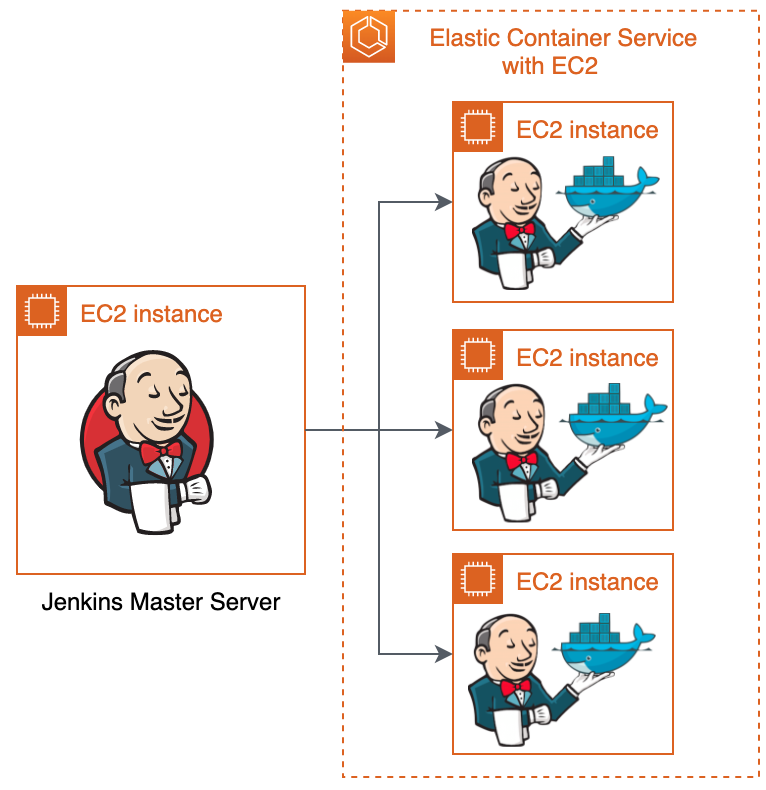
\includegraphics[width=\textwidth]{pics/jenkins-on-vm.png} % first figure itself
    \end{minipage}\hfill
    \begin{minipage}{0.54\textwidth}
        \centering
        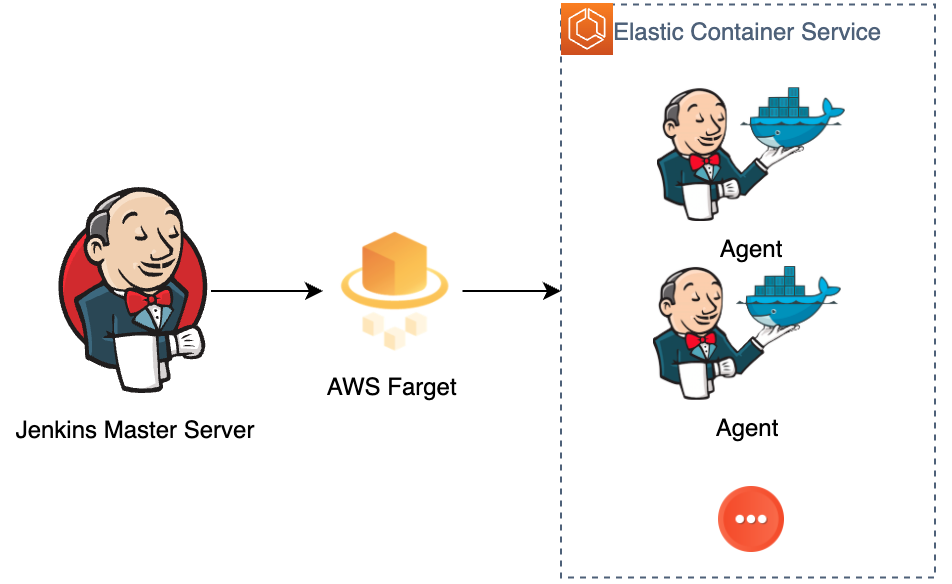
\includegraphics[width=\textwidth]{pics/jenkins-on-fargate.png} % second figure itself
    \end{minipage}
    \label{fig:ex1}
    \caption{Architecture diagram of the test Jenkins cluster with agents running in traditional virtual machines (left) and on ECS with AWS Fargate (right)}
\end{figure}
\subsubsection{Hardware}
The hardware of the instance that runs Jenkins agents is the independent variable that exposed to the change in the experiment.
\par
The experiments are conducted on Amazon Web Services (AWS). The hardware of Jenkins master node in both experiment groups is the same, which is EC2 instance of type t3.medium with 2 virtual CPU, 4 GB RAM and 30 GB disk. The EC2 instances as worker node is type t3.small, with 2 virtual CPU and 2GB RAM. Each EC2 instance can run 1 container at the same time.
\par
In the control group, which is the implementation we presented in CH4, the Jenkins agents run on AWS ECS powered by AWS Fargate. The virtual hardware resources that are allocated to each serverless container is 2 virtual CPU, and 2 GB of RAM. This makes sure that each container shares the same hardware resources as in another group, so the hardware will not affect the result.
\subsubsection{Software}
We maintain the same software setup in each group. The operation System for EC2 instance that runs Jenkins master node is Ubuntu Server 18.04. The version of Jenkins that runs on the server is 2.222.3. For connect ECS and Fargate which works as the Jenkins agents, we use Jenkins plugin "Amazon Elastic Container Service (ECS) / Fargate", version 1.34. The container in Fargate/EC2 for running the Checkout and Build steps is from our developed docker image which you can find at \footnote{https://hub.docker.com/r/dry1995/jnlp}. The docker image includes essential dependencies that will be used to build the Spring Boot application and the base image which allow container connects Jenkins master as an agent. The "Build" step in our pipeline uses Gradle (version: 6.2.1) as the build tool for the application, 
with openjdk 1.8.0.252 as Java virtual machine (JVM). The automated testing and code analysis is being integrated with this step, and being conducted by plugin of Gradle.
\par
To shows how does the 2 setups performance within the teams with different sizes, we run by run the different number of tasks parallel through the pipeline. This simulates the different team size that  and show the scalability when comes to the need for task parallelization in bigger organizations.

\subsection{Performance Properties and Evaluation}
We run the pipeline through 2 different setups, we will get the result of the following properties:
\begin{itemize}
    \item \textit{Runtime} describes the total time for finishing all the jobs. If the jobs runs in parallel, the runtime is from start of jobs until the end of the last finished job.
    \item \textit{Cost Structure} describes the daily cost of 2 setups under the same workload, within the same period.
    \item \textit{Resource Utilization} describes the average CPU/RAM usage for each instance during a single run of the pipeline.
\end{itemize}
\subsection{Result and Evaluation}
Here shows the result of this experiment. We also evaluate our experiment result by analysing the factors that lead to the results.
\subsubsection{Runtime}
We first compare the runtime of these 2 setups. Except test the runtime of single job runs with two setups respectively, we also test the runtime of each pipeline setup under different number jobs executed in parallel. The test result is depicted in Figure \ref{fig:runtime}.
\begin{figure}[h]
    \centering
    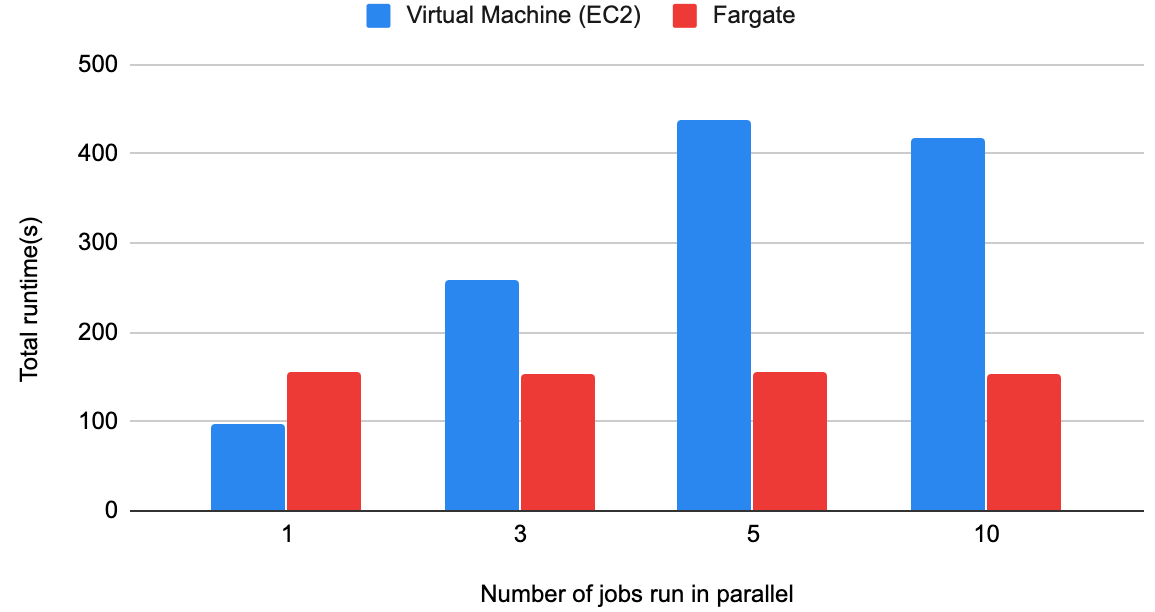
\includegraphics[width=0.99\textwidth]{pics/runtime.png}
    \caption{Runtime of Pipeline with Different Jenkins Agents}
    \label{fig:runtime}
\end{figure}
\begin{figure}[h]
    \centering
    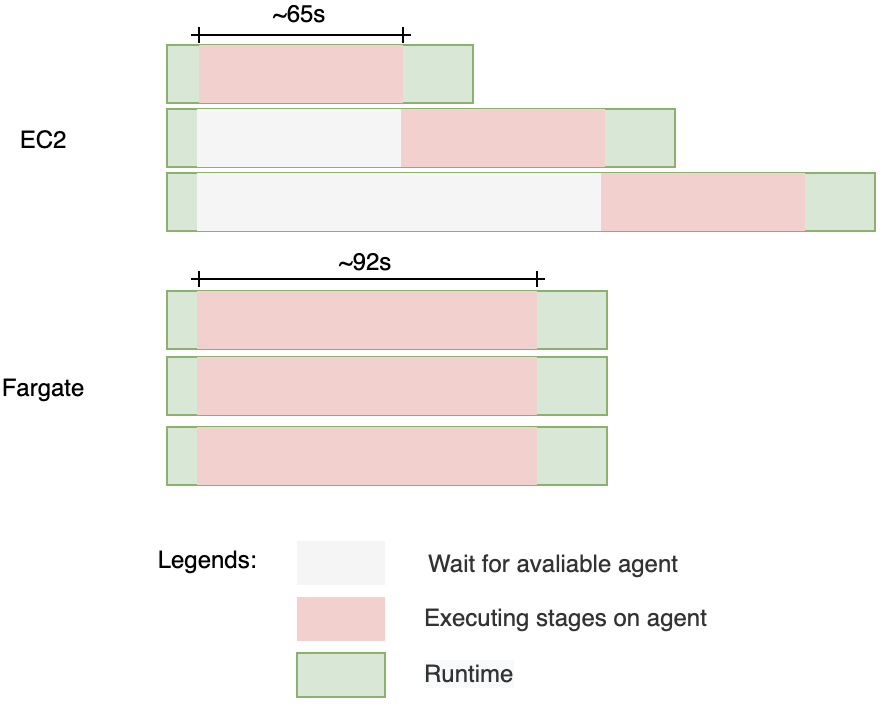
\includegraphics[width=0.99\textwidth]{pics/parallel.png}
    \caption{Execution Mode of Pipelines with Different Jenkins Agents}
    \label{fig:parallel}
\end{figure}
\par
The test result shows that, when comes to the execution of single task. The traditional VM has faster delivery speed over serverless solution (AWS Fargate). However, with the number of jobs that run in parallel increases, the total runtime on the traditional VM decrease. On the contract, on serverless solution(Fargate), the runtime remains almost the same.
\par
We analyse the reason behind this result, we found out that the longer runtime with the single job on Fargate is because the longer starting time of Jenkins agent. In EC2, the Jenkins will simply provision a Docker container within EC2 VM, and connect to the Jenkins master node. However in Fargate, the Jenkins can only connect to agent once AWS finishes the initialization of underlay infrastructure that runs the serverless container. This takes significantly longer time. This shows the one of the limitation of serverless computing (cold-start) that we mentioned in \ref{servlesslimitation}.

\par
When comes to parallel job execution, the performance of Fargate is significantly better. This is because in Fargate, each container runs on an independent instance on AWS's infrastructure, Therefore AWS provisions one Fargate instance for each running job. The independence between Fargate instance ensures the agent will not compete for resource. On the other hand, when we runs multiple agent in our EC2 instance, due to the limitation of resource, part of running jobs has to wait until the resource on EC2 instance available until they can start the execution. To further investigate the reason for the result, we observe the parallel execution mode when runs 3 jobs in parallel. Figure \ref{fig:parallel} shows the execution modes. We find that, the easy scalable character (mentioned in \ref{servlesslimitation}) helps the serverless suites better with the parallel task. The long wait time is the reason that makes the total runtime in EC2 much longer. 
\par
We also notice that in Figure 5.2, when parallel task reach 10, the EC2 runtime becomes shorter. This is because we set auto-scaling for our EC2 instance. So in the later part of our experiment, the EC2 scaled from 1 to 2 and then to 3. But even with 3 EC2 instances, only 3 jobs are allowed to run in parallel, while in Fargate is easy to have 10 jobs runs in complete parallel method. This because the scaling of EC2 VMs is much slower, because is heavier to create a VM than create a new Fargate instance. The other reason is the auto-scaling of EC2 VM is based on reaching certain resource utilization threshold, while in Fargate is based on one instance per container(Jenkins agent). Even we set the scaling policy of EC2 to a more aggressive patten, the AWS still more "hesitate" to create new instances compared with in the Fargate.
\subsubsection{Resource Utilization}
We compared the average resource utilization within containers that runs Jenkins agent in two setups. The data from AWS cloud watch shows the resource utilization rate is similar in these 2 setups. This is because the "run in same way regardless of host environment" \cite{WhatisaC60:online} feature of Docker container that we mentioned in \ref{docker}.
\begin{figure}[h]
    \centering
    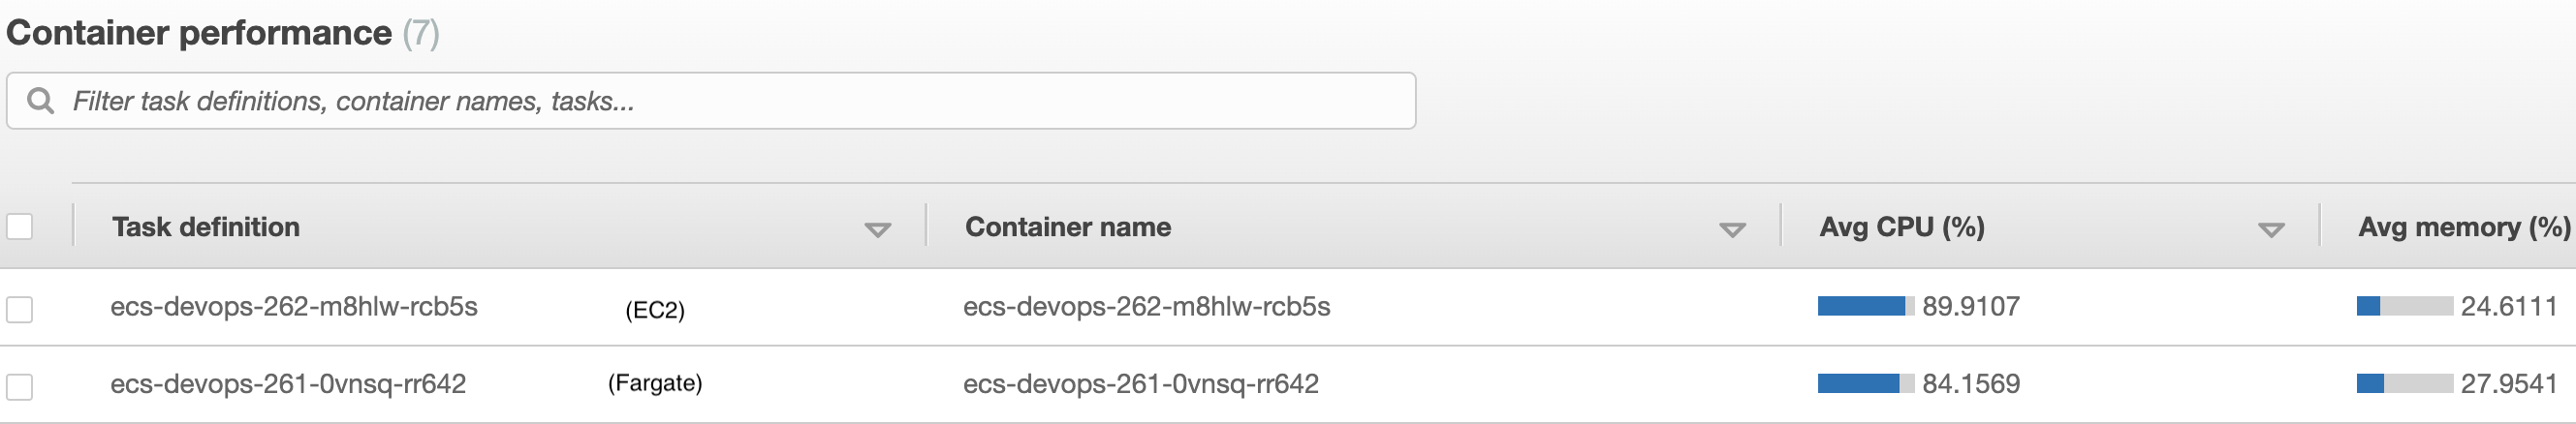
\includegraphics[width=0.99\textwidth]{pics/utilizationecs.png}
    \caption{The comparison of Resource Utilization}
    \label{fig:utilizationecs}
\end{figure}
\subsubsection{Cost Analysis}
The container orchestration service ECS itself is free of charge. We only pay for the resources we are using, which is Fargate or EC2 virtual machine.
\par
In AWS Fargate we pay only by resource we are using and the runtime. The price for Fargate service in EU(Stockholm) is \$0.004165 per GB RAM per hour plus \$0.0049 per vCPU per hour \footnote{https://aws.amazon.com/fargate/pricing/}. Thus in our experiment set-up (2vCPU, 2GB RAM) the price should be \$0.01813 per running agent for one hour's runtime.
In AWS EC2 our cost depends on type of VM we are using. The type of VM we use for running Jenkins agents is t3.small that costs \$0.0216 per hour \footnote{https://aws.amazon.com/ec2/pricing/on-demand/}. The Fargate-based Jenkins agent is cheaper than EC2-based agent.
\par
The pay-per-use characteristic of serverless service makes Fargate even more competitive in term of cost. The instance only up and run when the job is distributed by Jenkins master. One the job finished, the Fargate instance will be terminated immediately. However EC2 not so flexible due to the resource-utilization-based scaling policy. The EC2 instance is not scale in immediately after job finished, and user has to pay for the instance runtime before it gets terminated -- even there is no job running in EC2 instance any more.
\subsection{Conclusion}
In this experiment we compare the serverless (AWS Fargate) and non-serverless solution (EC2) for hosting distributed continuous delivery pipeline. The experiment shows that, the performance of serverless solution is worse when comes to single job execution, this is because the cold-start issue with serverless computing. However, in term of parallel job executing, the serverless solution has better performance over traditional VM. The cost of serverless solution is cheaper in AWS and the resource utilization is similar in both solutions.
\section{Experiment and Analysis of Managed DevOps Services}
For solving the RQ2, we compare the implementation of our design of two different the DevOps toolchain -- the non-integrated Jenkins based toolchain and the AWS DevOps toolchain implementation with AWS DevOps tooling.
\subsection{Test Task and System Description}
The first part of the experiment is similar with the last experiment, we deliver our case project through two DevOps toolchains. And we compare quantitative result from experiment.
The second part we are going to compare the functionality of these toolchains. However we will not compare all to functional, the scope of the comparison is limited around the actual problem we encounter during the implementation.  We will talk about the implementation difficulties, functionality limitation and flexibility.
\par
During the experiment we have set up as follows:
\paragraph{Hardware}
AWS DevOps tools allow us to select the hardware configuration for underlying computing resources. The configuration we chose is 2 virtual CPU and 3 GB RAM.
The Hardware configuration for Jenkins build agent is 2 virtual CPU and 4 GB RAM. We cannot set the RAM to 3 GB since AWS Fargate is not allowing \footnote{https://docs.aws.amazon.com/AmazonECS/latest/developerguide/task-cpu-memory-error.html} RAM to below 4GM when using 2 virtual CPU. However, we still allowed to set a additional software RAM limit to the build agent runs in Fargate agent, thus, we limit the RAM that a running build agent to 3 GB, which ensure both setup has identical hardware configuration.
\paragraph{Software}
The version of Jenkins that runs on the server is 2.222.3. We use Jenkins plugin ”Amazon Elastic Container Ser-vice (ECS) / Fargate”, version 1.34 for connect ECS and Fargate which works as the Jenkins agents. The Jenkins cluster has the same configuration as the last experiment. The build environment in both setup is the same, with Gradle (version:6.2.1) and JVM version is openjdk 1.8.0.252.
\subsection{Performance Properties and Evaluation Criteria}
We run the pipeline on these 2 different setups, we will get the result of the following properties:
\begin{itemize}
    \item \textit{Runtime} describes the total time for finishing all the jobs. If the jobs runs in parallel, the runtime is from start of jobs until the end of the last finished job.
    \item \textit{Cost Structure} describes the daily cost of 2 setups under the same workload, within the same period.
\end{itemize}
The resource utilization comparison is not available in the experiment since we cannot get the resources utilization in underlying hardware resource when running AWS DevOps tools.
\subsection{Quantitative Experiment Result and Evaluation}
\subsection{Functionality Comparison}
*** Should this subsection be moved to CH4? ***
